% ****** Start of file apssamp.tex ******
%
%   This file is part of the APS files in the REVTeX 4.1 distribution.
%   Version 4.1r of REVTeX, August 2010
%
%   Copyright (c) 2009, 2010 The American Physical Society.
% 
%   See the REVTeX 4 README file for restrictions and more information.
%
% TeX'ing this file requires that you have AMS-LaTeX 2.0 installed
% as well as the rest of the prerequisites for REVTeX 4.1
%
% See the REVTeX 4 README file
% It also requires running BibTeX. The commands are as follows:
%
%  1)  latex apssamp.tex
%  2)  bibtex apssamp
%  3)  latex apssamp.tex
%  4)  latex apssamp.tex
%
\documentclass[%
reprint,
superscriptaddress,
%groupedaddress,
%unsortedaddress,
%runinaddress,
%frontmatterverbose, 
% preprint,
%showpacs,preprintnumbers,
%nofootinbib,
%nobibnotes,
%bibnotes,
amsmath,amssymb,
aps,
prl,
%pra,
% prb,
%rmp,
%prstab,
%prstper,
%floatfix,
]{revtex4-1}

\usepackage{array}
\usepackage{graphicx}% Include figure files
\usepackage{dcolumn}% Align table columns on decimal point
\usepackage{bm}% bold math
\usepackage{amsmath}
%\usepackage{hyperref}% add hypertext capabilities
%\usepackage[mathlines]{lineno}% Enable numbering of text and display math
%\linenumbers\relax % Commence numbering lines

%\usepackage[showframe,%Uncomment any one of the following lines to test 
%%scale=0.7, marginratio={1:1, 2:3}, ignoreall,% default settings
%%text={7in,10in},centering,
%%margin=1.5in,
%%total={6.5in,8.75in}, top=1.2in, left=0.9in, includefoot,
%%height=10in,a5paper,hmargin={3cm,0.8in},
%]{geometry}

% % https://tex.stackexchange.com/questions/231191/algorithm-in-revtex4-1
\usepackage{algorithm}
\usepackage{algpseudocode}


\begin{document}

\title{Learning Atomistic Force Fields On-the-Fly with Bayesian Inference}

\author{Jonathan Vandermause}
\affiliation{Department of Physics, Harvard University, Cambridge, MA 02138, USA}
\affiliation{John A. Paulson School of Engineering and Applied
Sciences, Harvard University, Cambridge, MA 02138, USA}

\author{Steven B. Torrisi}
\affiliation{Department of Physics, Harvard University, Cambridge, MA 02138, USA}

\author{Simon Batzner}
\affiliation{Center for Computational Engineering, Massachusetts Institute of Technology, Cambridge, MA 02139, USA}

\author{Boris Kozinsky}
\affiliation{John A. Paulson School of Engineering and Applied
Sciences, Harvard University, Cambridge, MA 02138, USA}


\date{\today}

\begin{abstract}
\textit{Ab initio} molecular dynamics is a powerful tool for
accurately probing the dynamics of molecules and solids, but it is limited
to system sizes on the order of 1000 atoms and time scales on the order of
10 ps. We present a scheme for rapidly training a machine learning 
model of the interatomic force field that approaches the accuracy of \textit{ab initio} force calculations but can be applied to larger systems over longer time scales. Gaussian process models are trained “on-the-fly”, with density-functional theory calculations of the atomic forces performed whenever the model encounters chemical configurations outside of the training set. We demonstrate the flexibility of our approach by testing it on vacancy diffusion in bulk metals.
\end{abstract}

\maketitle

\section{Organization}

\begin{itemize}

\item Figure 1: Correlation between prediction error and out-of-sample variance. Train on a low temperature crystal and test at higher temperatures to systematically steer the model away from the training set. Establishing a correlation motivates the use of predictive variance for on-the-fly learning.

\item Algorithm 1: On-the-fly algorithm, including GP, MD, and DFT updates.

\item Figure 2: Number of DFT calls vs simulation time. A sharp increase should be observed when new phases are introduced.

\item Table 1: Performance of FLARE compared with state-of-the art EAM and ML models. Models tested on independent \textit{ab initio} MD runs. MAEs and mean absolute force components reported in eV/A.

\item Figure 3: Validation of the force field. Parity plots, radial distribution function, and activation profiles should agree with \textit{ab initio} calculations.

\item Supplementary Figure 1: Numerical demonstration of energy conservation. Plot the RMS energy fluctuations against the time step squared and check that the resulting graph is linear \cite{allen2017computer}.

\item Supplementary Figure 2: Justification of cutoff selection. Plot likelihood, noise parameter, and out-of-sample error vs. cutoffs.

\item Supplementary Table 1: Table of formulas for calculating kernels.

\item Supplementary Table 2: Justification of quadratic cutoff. Record log likelihood for different cutoffs (cosine, hard, quadratic).

\end{itemize}

\section{Supplementary Information}

\subsection{Covariant kernels for direct force prediction}
The total energy $E$ of a system of atoms in a periodic cell is modelled as a sum over two- and three-body contributions,
\begin{equation}
E = \sum_{ij} \varepsilon_{ij} + \sum_{ijk} \varepsilon_{ijk},
\end{equation}
where the sums range over all unique pairs and triplets of atoms containing at least one atom from the unfolded primary cell. In practice, the sums are truncated by considering local atom-centered environments surrounding each atom in the primary cell and neglecting contributions from atoms beyond a chosen cutoff distance from the central atom. The energy may then be expressed as
\begin{equation}
  E = \sum_{i} \left( \frac{1}{2} \sum_{j \in \rho_i} \varepsilon_{ij} + \frac{1}{3} \sum_{j, k \in \rho_i} \varepsilon_{ijk} \right),
\end{equation}
where $\rho_i$ denotes the local environment of atom $i$ containing all atoms within the cutoff sphere and the fractional factors take care of multiple counting due to the repeated appearance of bonds and triplets in neighboring environments. This may be written more compactly as
\begin{equation}
E = \sum_i \varepsilon_i,
\end{equation}
where $\varepsilon_i \equiv \frac{1}{2} \sum_{j \in \rho_i} \varepsilon_{ij} + \frac{1}{3} \sum_{j, k \in \rho_i} \varepsilon_{ijk}$ may be viewed as the local energy of atom $i$.

In Gaussian process models, the covariance between targets is set equal to a kernel or similarity measure between inputs. The covariance between total energy observations $E_l, E_m$ of two distinct structures $\sigma_l, \sigma_m$ may be written as
\begin{equation}
\left\langle E_l E_m \right\rangle = \sum_{i \in \sigma_l} \sum_{j \in \sigma_m} \langle \varepsilon_i \varepsilon_j \rangle,
\end{equation}
where the covariance between local energies is
\begin{equation}
\langle \varepsilon_i \varepsilon_j \rangle = \frac{1}{4} \sum_{n \in \rho_i} \sum_{p \in \rho_j} \langle \varepsilon_{i n} \varepsilon_{j p} \rangle + \frac{1}{9} \sum_{n, q \in \rho_i} \sum_{p, r \in \rho_j} \langle \varepsilon_{inq} \varepsilon_{jpr} \rangle.
\end{equation}
Letting $F_{i\xi} = - \frac{d E}{d \xi_i}$ denote the force on atom $i$ along Cartesian component $\xi$, the covariance between force observations may be written as
\begin{equation}
  \langle F_{i\xi} F_{j \chi} \rangle =  \sum_{n \in \rho_i} \sum_{p \in \rho_j} \frac{\partial^2}{\partial \xi_i \partial \chi_j} \langle \varepsilon_{i n} \varepsilon_{j p} \rangle +  \sum_{n, q \in \rho_i} \sum_{p, r \in \rho_j} \frac{\partial^2}{\partial \xi_i \partial \chi_j} \langle \varepsilon_{inq} \varepsilon_{jpr} \rangle,
\end{equation}
where here the fractional factors do not appear as the sums are restricted to the local environments of atoms $i$ and $j$. This is convenient in practice, as it allows local information about individual atoms to be used at test time without having to store the atomic environments of all the other atoms in the structure.

In order to infer energies from force observations, it is necessary to consider the covariance between energies and forces.

\newpage

\begin{figure}
	\centering
	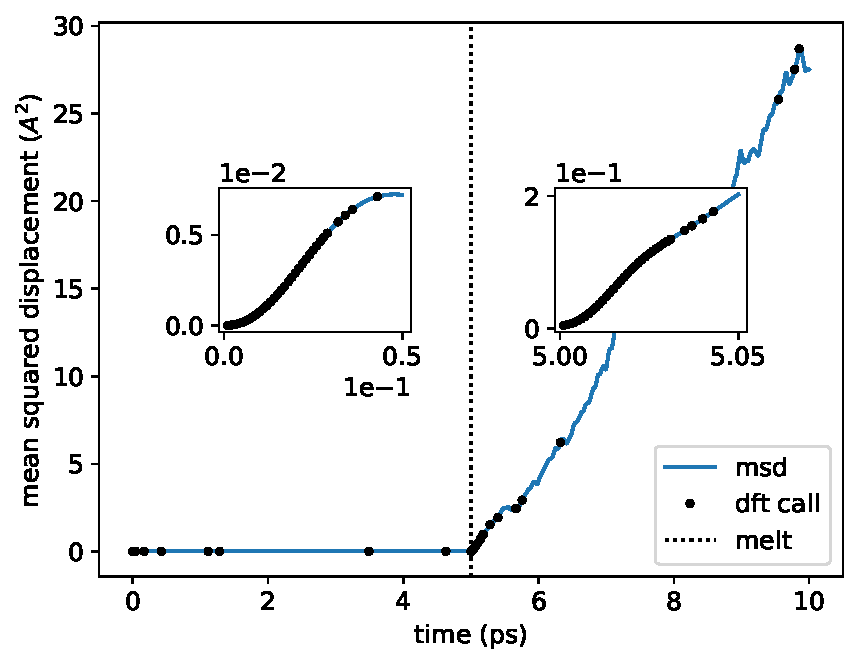
\includegraphics[width=3.4in]{melt_msd_3.pdf}
	\caption{On-the-fly learning of an aluminum force field at multiple temperatures.}
\end{figure}

\begin{figure}
	\centering
	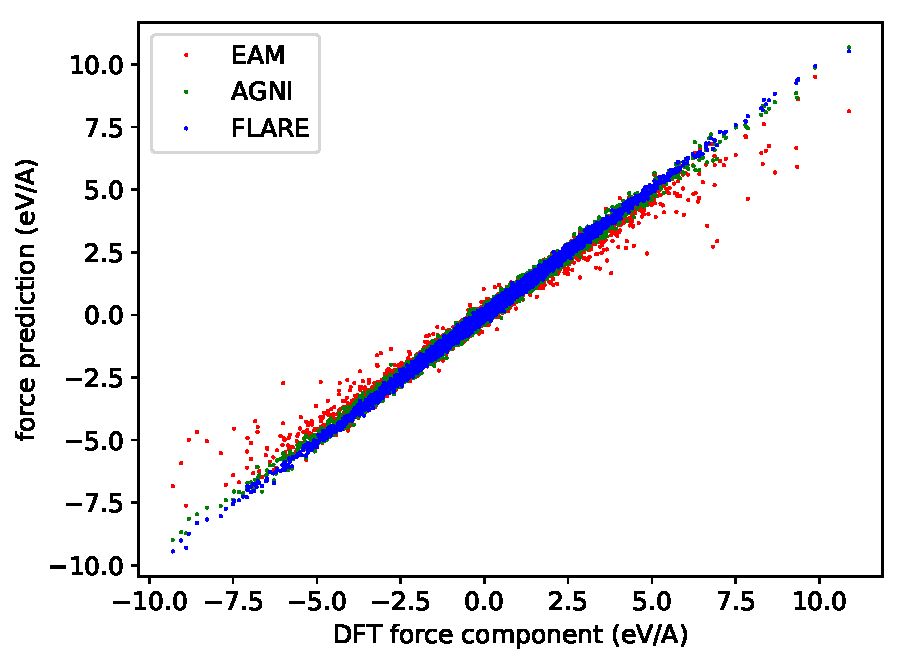
\includegraphics[width=3.4in]{parity_liquid.pdf}
	\caption{Mean square displacement of aluminum melt.}
\end{figure}

\begin{figure}
	\centering
	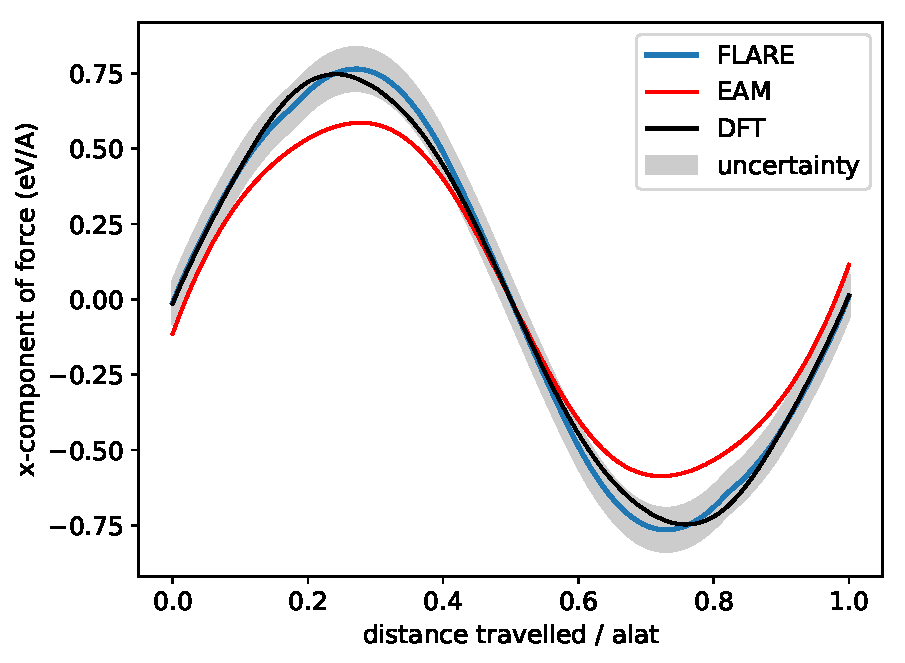
\includegraphics[width=3.4in]{vacancy_act.pdf}
	\caption{Mean square displacement of aluminum melt.}
\end{figure}

\begin{figure}
	\centering
	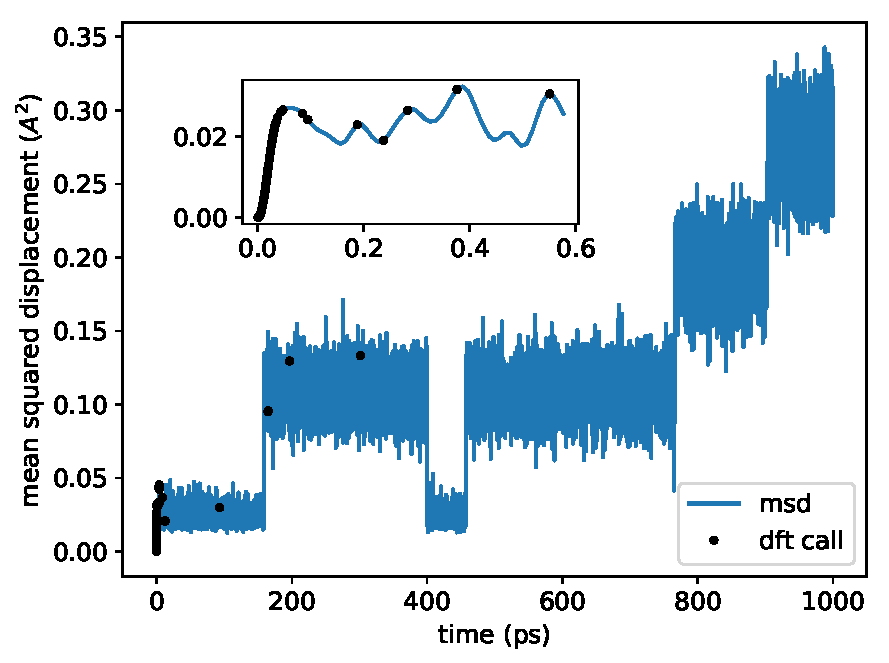
\includegraphics[width=3.4in]{vacancy_msd.pdf}
	\caption{Mean square displacement of aluminum melt.}
\end{figure}

\begin{figure}
	\centering
	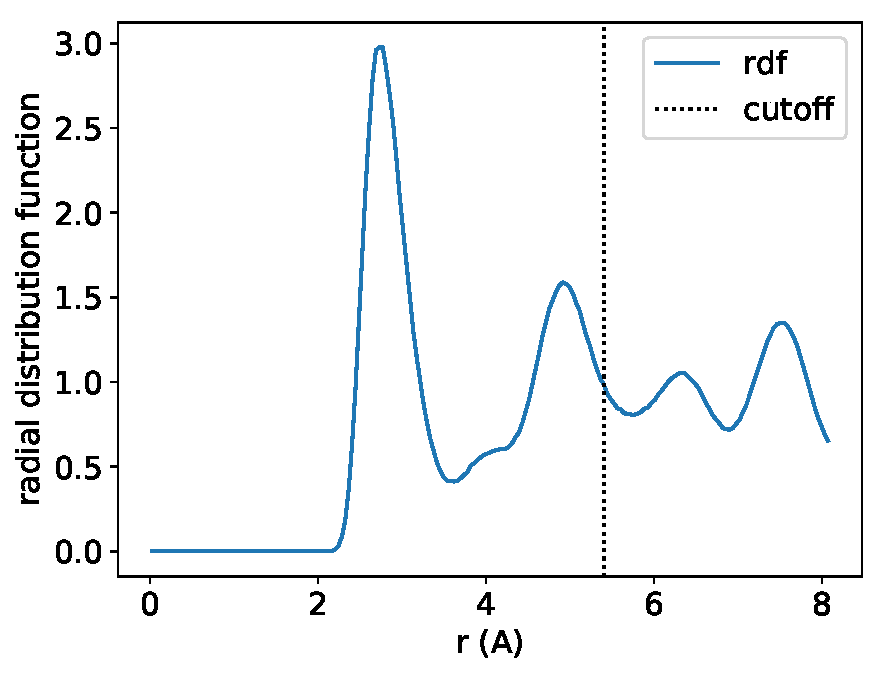
\includegraphics[width=3.4in]{rdf.pdf}
	\caption{RDF of Al melt.}
\end{figure}

% https://en.wikibooks.org/wiki/LaTeX/Tables
\begin{table}
\begin{tabular}
{ |p{1.4cm}|| >{\centering} p{1.4cm}| >{\centering} p{1.4cm}| >{\centering} p{1.4cm}| p{1.4cm} <{\centering}|  }
	% \hline
	% \multicolumn{4}{|c|}{Model Error} \\
	\hline
	 & Solid & Liquid & Slab & Vacancy \\
	\hline
	OTF & & & & \\
	\hline
	EAM & & & & \\
  \hline
	AGNI & & & & \\
	\hline
\end{tabular}
\caption{On-the-fly force field error compared to a recent EAM potential.}
\end{table}

% https://en.wikibooks.org/wiki/LaTeX/Algorithms#Typesetting_using_the_algorithmic_package
\begin{algorithm}[H]
  \caption{Active Learning of Atomistic Force Fields}
  \label{EPSA}
   \begin{algorithmic}[1]
   \Require initial structure (positions, velocities, periodic cell)
   \Require initial GP model (kernel and hyperparameters)
   \Require $\Delta t$: molecular dynamics time step
   \Require $T$: total simulation time
   \Require $\mathcal{U}$: initial uncertainty threshold
   \State Initialize time: t = 0
   \While {$t < T$}
   \State predict forces and uncertainties with GP model
   \If {uncertainty above threshold}
   \State compute forces with DFT
   \State add highest uncertainty atom to training set
   \State update GP hyperparameters
   \State update structure with DFT forces
   \Else
   \State update structure with GP forces
   \EndIf
   \State update time: $t = t + \Delta t$
   \EndWhile
   \end{algorithmic}
\end{algorithm}

\begin{center}
    \begin{table}
    \begin{tabular}{ |c|c|c| } 
     \hline
     Energy Kernel & $k_{\text{inv}}$ & $\sigma^2 \sum_{c, p} k f_{\text{cut}}(\vec{d}_c) f_{\text{cut}}(\vec{d}_p)$ \\ 
     \hline
     - & $k$ & $\exp\left( - \frac{||\vec{d}_c - \vec{d}_p ||^2}{2 \ell^2} \right)$\\
     \hline
     - & $\vec{d}^{(2)}$ & $(r_{i_1})$ \\
     \hline
     - & $\vec{d}^{(3)}$ & $(r_{i_1}, r_{i_2}, r_{i_1, i_2})$ \\
     \hline
    Force Kernel & $\frac{\partial^2 k_{\text{inv}}}{\partial \xi_i \partial \chi_j}$ & $\sigma^2 \sum_{c, p} (k_0 + k_1 + k_2 + k_3)$ \\ 
     \hline
     - & $k_0$ & $k \frac{\partial f_{\text{cut}}(\vec{d}_c)}{\partial \xi_i} \frac{\partial f_{\text{cut}}(\vec{d}_p)}{\partial \chi_j}$ \\ 
     \hline
     - & $k_1$ & $\frac{\partial k}{\partial \xi_i} f_{\text{cut}}(\vec{d}_c) \frac{\partial f_{\text{cut}}(\vec{d}_p)}{\partial \chi_j}$ \\ 
     \hline
     - & $k_2$ & $\frac{\partial k}{\partial \chi_j} \frac{\partial f_{\text{cut}}(\vec{d}_c)}{\partial \xi_i} f_{\text{cut}}(\vec{d}_p)$ \\ 
     \hline
     - & $k_3$ & $\frac{\partial^2 k}{\partial \xi_i \partial \chi_j} f_{\text{cut}}(\vec{d}_c) f_{\text{cut}}(\vec{d}_p)$ \\ 
     \hline
     - & $\frac{\partial k}{\partial \xi_i}$ & $\frac{k B_1}{\ell^2}$ \\ 
     \hline
     & $B_1$ & $\sum_{q=1}^{N-1} \frac{(r_{i_q} - r_{j_q})\xi_{i_q}}{r_{i_q}}$ \\
     \hline
     - & $\frac{\partial k}{\partial \chi_j}$ &  $-\frac{k B_2}{\ell^2}$ \\ 
     \hline
    - & $B_2$ & $\sum_{q=1}^{N-1} \frac{(r_{i_q} - r_{j_q})\chi_{j_q}}{r_{j_q}}$ \\
     \hline
     - & $\frac{\partial^2 k}{\partial \xi_i \chi_j}$ & $\frac{k}{\ell^4} \left(A \ell^2 -B_1 B_2 \right)$\\ 
     \hline
     - & $A$ & $\sum \frac{\xi_{i_q} \chi_{j_q}}{r_{i_q} r_{j_q}}$ \\
     \hline
     $\ell$ Derivative & $\frac{\partial^3 k_{\text{inv}}}{\partial \ell \partial \xi_i \partial \chi_j}$ & $\sigma^2 \sum_{c, p} \left(\frac{\partial k_0}{\partial \ell} + \frac{\partial k_1}{\partial \ell} + \frac{\partial k_2}{\partial \ell} + \frac{\partial k_3}{\partial \ell}\right)$ \\
     \hline
     - & $\frac{\partial k}{\partial \ell}$ & $\frac{k ||\vec{d}_c - \vec{d}_p||^2}{l^3}$ \\
     \hline
     - & $\frac{\partial^2 k}{\partial \ell \partial \xi_i}$ & $B_1 \left( \frac{1}{\ell^2} \frac{\partial k}{\partial \ell} - \frac{2 k}{\ell^3} \right)$ \\
     \hline
     - & $\frac{\partial^2 k}{\partial \ell \partial \chi_j}$ & $-B_2 \left( \frac{1}{\ell^2} \frac{\partial k}{\partial \ell} - \frac{2 k}{\ell^3} \right)$ \\
     \hline
     - & $\frac{\partial^3 k}{\partial \ell \partial \xi_i \partial \chi_j}$ & $\left( A \ell^2 - B_1 B_2 \right) \left( \frac{\partial k}{\partial \ell} \frac{1}{\ell^4} - \frac{4 k}{\ell^5} \right) + \frac{2 k A}{\ell^3}$ \\
     \hline
     $\sigma$ Derivative & $\frac{\partial^3 k_{\text{inv}}}{\partial \sigma \partial \xi_i \partial \chi_j}$ & $2 \sigma \sum_{c, p} (k_0 + k_1 + k_2 + k_3)$ \\
     \hline
    \end{tabular}
    \caption{Quantities used to calculate the smoothed $N$-body force kernel and its derivatives.}
\end{table}
\end{center}


\bibliography{otf.bib}

\end{document}
%
% ****** End of file apssamp.tex ******